\documentclass[10pt,usenames,dvipsnames]{beamer}
\usetheme{CambridgeUS}
%\usetheme{Boadilla}
\definecolor{myred}{RGB}{163,0,0}
%\usecolortheme[named=`blue]{structure}
\usecolortheme{dove}
\usefonttheme[]{professionalfonts}
\usepackage[english]{babel}
\usepackage{amsmath,amsfonts,amssymb}
\usepackage{xcolor}
\usepackage{tikz}
\usepackage{pgfplots}
\pgfplotsset{compat=newest,compat/show suggested version=false}
\usetikzlibrary{arrows,shapes,calc,backgrounds}
\usepackage{bm}
\usepackage{textcomp}
\usepackage{gensymb}
\usepackage{verbatim}
\usepackage{paratype}
\usepackage{mathpazo}
\usepackage{listings}
\usepackage{csvsimple}

\newcommand{\cov}{\mathsf{cov}}
\newcommand{\corr}{\mathsf{corr}}
\newcommand{\var}{\mathsf{Var}}
\newcommand{\plim}{\mathrm{plim\ }}
\newcommand{\E}{\mathsf{E}}
\newcommand{\Est}{\mathsf{Est.Var}}
\newcommand{\Asy}{\mathsf{Asy.Var}}
\newcommand{\Esta}{\mathsf{Est.Asy.Var}}
\newcommand{\tr}{\mathrm{tr}}
\newcommand{\Prob}{\mathrm{Prob}}
\newcommand{\Med}{\mathsf{Med}}
\newcommand{\rank}{\mathsf{rank}}
\newcommand{\argmin}{\mathsf{arg\,min}}

\newcommand{\cc}[1]{\texttt{\textcolor{blue}{#1}}}

\definecolor{ttcolor}{RGB}{0,0,1}%{RGB}{163,0,0}

% Number theorem environments
\setbeamertemplate{theorem}[ams style]
\setbeamertemplate{theorems}[numbered]

% Reset theorem-like environments so that each is numbered separately
\usepackage{etoolbox}
\undef{\definition}
\theoremstyle{definition}
\newtheorem{definition}{\translate{Definition}}

\definecolor{ttcolor}{RGB}{0,0,1}%{RGB}{163,0,0}
\definecolor{mygray}{RGB}{248,249,250}

% Change colours for theorem-like environments
\definecolor{mygreen1}{RGB}{0,96,0}
\definecolor{mygreen2}{RGB}{229,239,229}
\setbeamercolor{block title}{fg=white,bg=mygreen1}
\setbeamercolor{block body}{fg=black,bg=mygreen2}

\lstdefinestyle{numbers}{numbers=left, stepnumber=1, numberstyle=\tiny, numbersep=10pt}
\lstdefinestyle{MyFrame}{backgroundcolor=\color{yellow},frame=shadowbox}

\lstdefinestyle{rstyle}%
{language=R,
	basicstyle=\footnotesize\ttfamily,
	backgroundcolor = \color{mygray},
	commentstyle=\slshape\color{green!50!black},
	keywordstyle=\bfseries\color{blue!50!black},
	identifierstyle=\color{blue},
	stringstyle=\color{orange},
	%escapechar=\#,
	rulecolor = \color{mygray}, 
	showstringspaces = false,
	showtabs = false,
	tabsize = 2,
	emphstyle=\color{red},
	frame = single} 

\setbeamertemplate{navigation symbols}{}

\lstset{language=R,frame=single}

\AtBeginSection{\frame{\sectionpage}}

% Remove Section 1, Section 2, etc. as titles in section pages
\defbeamertemplate{section page}{mine}[1][]{%
	\begin{centering}
		{\usebeamerfont{section name}\usebeamercolor[fg]{section name}#1}
		\vskip1em\par
		\begin{beamercolorbox}[sep=12pt,center]{part title}
			\usebeamerfont{section title}\insertsection\par
		\end{beamercolorbox}
	\end{centering}
} 

\setbeamertemplate{section page}[mine]  

\hypersetup{colorlinks, urlcolor=blue, linkcolor = myred}

\title{R406: Applied Economic Modelling with Python}    
\subtitle{\textcolor{myred}{Ordinary Differential Equations of First, Second, and Higher Order}}
\author[Kaloyan Ganev,  Andrey Vassilev]{Kaloyan Ganev (main author) \\
	Andrey Vassilev (minor modifications)}

\date{} 

\begin{document}
\maketitle

\begin{frame}[fragile]
\frametitle{Lecture Contents}
\tableofcontents
\end{frame}

\section{Introduction}
\subsection{Definition of Concepts}
\begin{frame}[fragile]
	\frametitle{From difference to differential equations} % Based on Ph. Michel, Cours de mathématiques pour économistes
	\framesubtitle{}
		\begin{itemize}
		\item To provide an intuitive motivation for differential equations, consider a situation where we have a quantity of interest $ y(t) $ that evolves in  continuous time
		\item However, this quantity is observed at discrete points in time and we can choose the step between adjacent observations
		\item Given a time step $ h $, our observations are recorded at times $\tau,~ \tau+h,~ \tau+2h,~\tau+3h,~ \ldots$
		\item The above can always be re-labelled to ``lose'' the time step by setting \[ t+k = \tau + kh, ~ k=0,1,2,\ldots \]
		
	\end{itemize}
\end{frame}

\begin{frame}[fragile]
	\frametitle{From difference to differential equations (2)}
	\framesubtitle{}
	\begin{itemize}
		\item Assume that such a process can be described by a difference equation of the form
		\[ \dfrac{1}{h}(y_{s+1}-y_s) = f(y_s) \] i.e.
		\[ \dfrac{1}{h}(y_{t+h}-y_t) = f(y_t) \]
		\item If we let the time step $ h $ tend to 0, i.e. we observe with increasing frequency, the left-hand side will tend to the derivative $ \dot{y}(t) := \dfrac{dy(t)}{dt} $
		\item In the limit, the recursive relationship will change to a relationship the form \[ \dot{y}(t) = f(y(t)) \]
		\item The last expression is a relationship between an unknown function $ y(t) $ and its first derivative
	\end{itemize}
\end{frame}



\begin{frame}[fragile]
\frametitle{What is a Differential Equation?}
\begin{definition}
	A differential equation is an equation that relates an unknown function with one or more of its derivatives.
\end{definition}
\begin{itemize}
	\item Note that a differential equation relates to an \textit{unknown function} not to an \textit{unknown number}
	\item Note that such an equation can have one or more variables, constants, etc.
	\item Given two variables $x$ and $y$, the general form of a differential equation in those two variables could be:
	\[
		\dfrac{dy}{dx} = f(x,y)
	\]
	\item We will be considering only variables that are functions of time, therefore we can speak equivalently of \textit{dynamic systems}
	\item Time itself (denoted by $t$) is considered a continuous variable
\end{itemize}
\end{frame}

\begin{frame}[fragile]
\frametitle{Ordinary Differential Equations}
\begin{definition}
	An ordinary differential equation (ODE) is a differential equation that includes the derivatives of only one function of time.
\end{definition}
\begin{itemize}
	\item Example:
	\[
		\dot{x} = ax + b
	\]
	This is not an ODE:
	\[
		\dot{x} = ax + b + \dot{y} + cy
	\]
	\item Note that we will be using Newton's \textit{dot notation} of derivatives
	\item Just to be aware: equations including the partial derivatives of unknown functions of more than one variable are called \textit{partial differential equations}
\end{itemize}
\end{frame}

\begin{frame}[fragile]
\frametitle{ODE Order}
\begin{definition}
	The order of an ODE is defined by the order of the highest derivative present in the equation.
\end{definition}
\begin{itemize}
	\item Examples:
	\[
		\begin{array}{lcl}
			\dot{x} = ax \textrm{ (first-order ODE)}\\
			\quad\\
			\ddot{x} = \dot{x} + z \textrm{ (second-order ODE)}\\
			\quad\\
			\textrm{etc.}
		\end{array}
	\]
\end{itemize}
\end{frame}

\begin{frame}[fragile]
\frametitle{Linear vs. Non-linear ODE}
\begin{definition}
	A linear ODE satisfies the following:
	\begin{itemize}
	 	\item The dependent variable and its derivatives appear to the power of one only
	 	\item There are no products of the dependent variable and/or its derivatives in the equation
	 	\item There are no transcendental functions\footnote{Functions that cannot be expressed in terms of a finite sequence of the algebraic operations of addition, multiplication, and root extraction.} of the dependent variable and/or its derivatives
	 \end{itemize} 
\end{definition}
\begin{itemize}
	\item A non-linear ODE is one not fitting the above definition
	\item Example:
	\[
		\dot{x} = \dfrac{1}{t} -2\cos(x)
	\]
\end{itemize}
\end{frame}

\begin{frame}[fragile]
\frametitle{ODE: Constant vs. Variable Coefficients}
\begin{itemize}
	\item Consider the general form of an $n$th-order linear ODE:
	\[
		a_{0}(t)\dfrac{d^{n}x}{dt^{n}} + a_{1}(t)\dfrac{d^{n-1}x}{dt^{n-1}} + \ldots + a_{n}(t)x = g(t) \quad (*)
	\]
	where $g(t)$ is some function of time
	\item Some equations might imply coefficient which themselves are functions of $t$ 
	\item Those are equations with \textit{variable coefficients} 
	\item With some exceptions, we will usually work with \textit{constant-coefficients equations} which means that all $a_{i} = const,i = 0,\ldots,n$
\end{itemize}
\end{frame}

\begin{frame}[fragile]
\frametitle{Homogeneous vs. Non-homogeneous ODE}
\begin{definition}
	In $(*)$, if $g(t) \equiv 0$, then the equation is called \textit{homogeneous}.
\end{definition}
\begin{itemize}
	\item Example:
	\[
		\dot{x} = ax
	\]
	\item Otherwise, the equation is called \textit{non-homogeneous}
		\item Example:
	\[
		\dot{x} = ax + b, \quad b \neq 0
	\]
\end{itemize}
\end{frame}

\begin{frame}[fragile]
\frametitle{Autonomous vs. Non-autonomous ODE}
\begin{definition}
	\textit{Autonomous} ODE are equations in which time is not explicitly present as an independent variable.	
\end{definition}
\begin{itemize}
	\item Therefore, such equations are also popular as \textit{time-invariant} ODE
	\item The equations in the previous slide, for example, are autonomous
	\item A non-autonomous one would be for instance:
	\[
		\dot{x} = ax + be^{-t}, \quad b \neq 0
	\]
\end{itemize}
\end{frame}

\subsection{Solutions to Linear ODE}
\begin{frame}[fragile]
\frametitle{Solutions to Linear ODE}
\begin{itemize}
	\item Take $(*)$ once again
\end{itemize}
\begin{definition}
	A solution to this equation (if it exists) in an interval $I = \{t: a < t < b\}$ is the $n$-times differentiable function $\phi(t)$ which is defined on $I$ and is such that when substituted in $(*)$, satisfies it exactly over the whole interval.
\end{definition}
\begin{enumerate}
	\item The graph of the solution of $(*)$ is called the \textit{solution curve} (or \textit{integral curve})
	\item The set of all solutions is called the \textit{general solution}
	\item Any specific solution that satisfies the differential equation is called a \textit{particular solution}
\end{enumerate}
\end{frame}

\begin{frame}[fragile]
\frametitle{Explicit and Implicit Solutions; Graphical Solutions}
\begin{itemize}
	\item Some equations have \textit{explicit solutions}, i.e. the unknown functions can be expressed directly in terms of the independent variable(s)
	\item Sometimes, however, this is impossible, therefore solutions could also be present as \textit{implicit} ones
	\item Graphical solution can be \textit{quantitative} if the exact values of the function are known
	\item If the exact values are unknown but could be reasonably approximated, the solutions are called \textit{qualitative}
\end{itemize}
\end{frame}

\subsection{The Initial-Value Problem}
\begin{frame}[fragile]
\frametitle{Initial-Value Problems}
\begin{itemize}
	\item As far as solutions imply integration, finding the unknown function(s) is in fact finding a family of functions
	\item Often we are interested in a particular member of this family that passes through a specified point
	\item The latter specifies the \textit{initial-value problem}
	\item Initial-value problems are common in economics (example: the path of the capital stock)
\end{itemize}
\end{frame}

\begin{frame}[fragile]
\frametitle{Qualitative Theory}
\begin{itemize}
	\item Not all differential equations have explicit solutions
	\item Such are not always needed, however
	\item It is enough to know some of the properties of the dynamic system
	\item Qualitative theory offers the necessary existence and uniqueness theorems, etc.
\end{itemize}
\end{frame}

\begin{frame}[fragile]
\frametitle{Slope Fields}
\begin{itemize}
	\item Also called \textit{direction diagrams}
	\item They are stylized graphical representations of all solutions to a dynamic system
	\item For example, for the equation 
	\[
		\dot{y} = x - y 
	\]
	we have
\end{itemize}
\begin{center}
	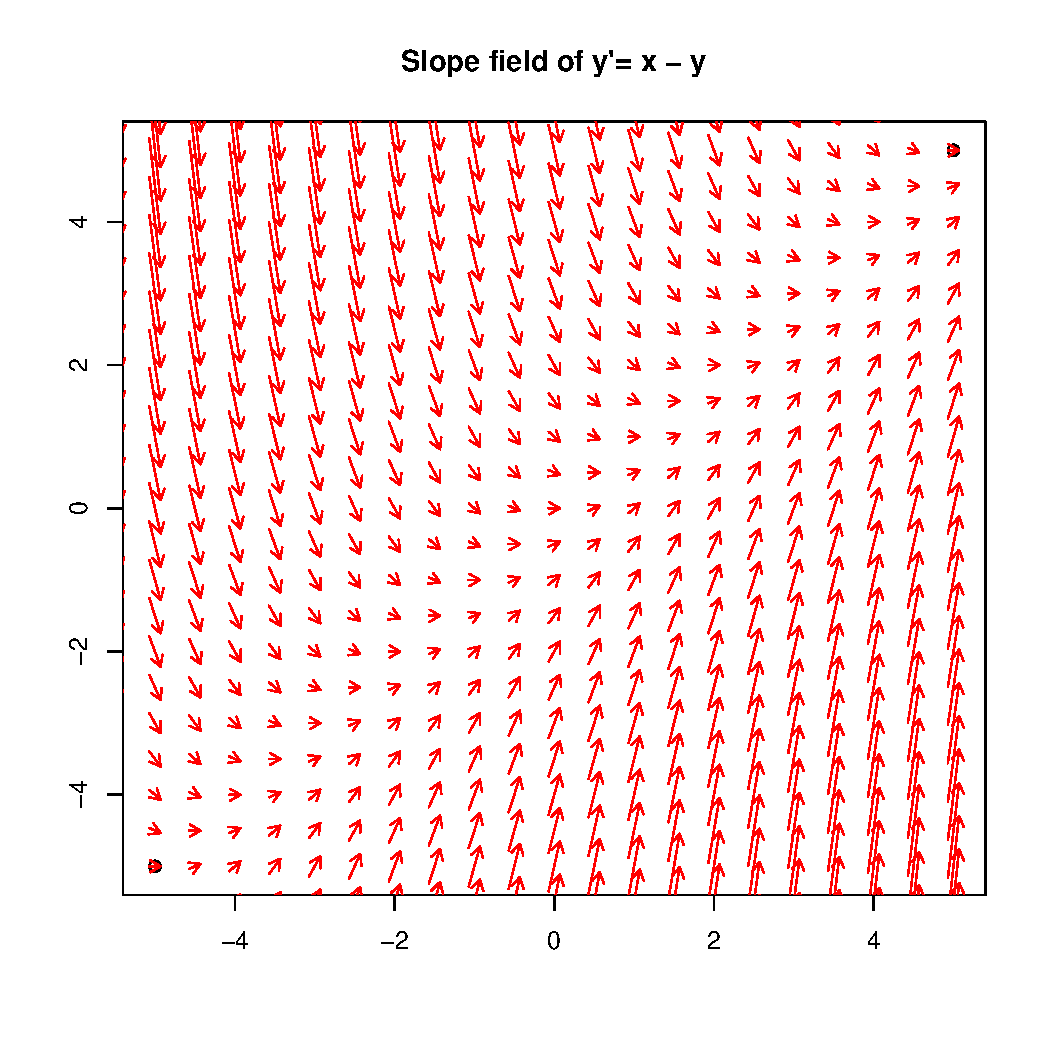
\includegraphics[scale=0.3]{./graphs/fig1.pdf}
\end{center}

\end{frame}

\section{Separable Equations}
\begin{frame}[fragile]
\frametitle{Separable Equations}
\begin{itemize}
	\item Suppose we have the following first-order ODE:
	\[
		\dot{x} = F(x,t) 
	\]
	\item Suppose also that $F(x,t)$ can be written as the product of two functions, one of $t$ only, and one of $x$ only:
	\[
		\dot{x} = f(t)\cdot g(x)\quad (**)
	\]
\end{itemize}

\begin{definition}
	Equations that can be represented as the product of such functions are called \textit{separable}.
\end{definition}
\end{frame}

\begin{frame}[fragile]
\frametitle{Separable Equations (2)}
\begin{itemize}
	\item Examples:
	\[
		\begin{array}{lcl}
			\dot{x} = -2tx^{2}\quad (separable)\\
			\quad\\
			\dot{x} = -2t + x^{2}\quad (non-separable)\\
		\end{array}
	\]
	\item If $g(x)$ has a zero at $x = a$ (i.e. $g(a) = 0$), then $x(t) \equiv a$ is a particular solution to $(**)$
	\item Why? Because $\dot{x}(t) = \dot{a} = 0$ (LHS) and also $f(t)\cdot g(x) = f(t)\cdot g(a) = 0$ (RHS)
\end{itemize}
\end{frame}

\begin{frame}[fragile]
\frametitle{Separable Equations: Solution Steps}
\begin{enumerate}
	\item Write $(**)$ as follows:
	\[
		\dfrac{dx}{dt} = f(t)\cdot g(x)
	\]
	\item Separate variables:
	\[
		\dfrac{dx}{g(x)} = f(t)dt
	\]
	\item Integrate:
	\[
		\int \dfrac{dx}{g(x)} = \int f(t)dt
	\]
	\item Evaluate integral, find solution (explicit or implicit)
	\item Every zero $x = a$ of $g(x)$ gives a particular solution $x(t) \equiv a$
\end{enumerate}

(We will solve some examples.)
\end{frame}

\begin{frame}[fragile]
	\frametitle{Solved Examples of Separable Equations}
	\begin{itemize}
		\item \textcolor{OliveGreen}{Example 1:} Solve the equation:
		\[
			\dfrac{dx}{dt} = \dfrac{1}{x^{2}}
		\]
		
		\color{red}
		\item Solution:
		\[
			\begin{array}{lcl}
				x^{2}\,dx = dt\\
				\quad\\
				\displaystyle \int x^{2}\,dx = \int dt\\
				\quad\\
				\dfrac{x^{3}}{3} = t + C \Rightarrow x = \sqrt[3]{3(t + C)}
			\end{array}
		\]
		
		Check: $ \dfrac{dx}{dt} = \dfrac{1}{3}\cdot[3(t + C)]^{-2/3}\cdot 3 = \dfrac{1}{\left(\sqrt[3]{3(t + C)}\right)^{2}} $
	\end{itemize}
\end{frame}

\begin{frame}[fragile]
	\frametitle{Solved Examples of Separable Equations (2)}
	\begin{itemize}
		\item \textcolor{OliveGreen}{Example 2:}\footnote{Borrowed from Shone (2002), p. 48.} Radioactive decay of atomic particles:
		\[
			\dfrac{dn}{dt} = -\lambda n,\quad \lambda > 0
		\]
		where $ \dfrac{dn}{dt} $ is the number of atoms that degenerate per unit of time, and $ \lambda $ is the decay constant 
		
		\color{red}
		\item Solution:
		\[
			\begin{array}{lcl}
				\dfrac{dn}{n} = -\lambda\, dt\\
				\quad\\
				\displaystyle \int \dfrac{dn}{n} = -\lambda\int\, dt
			\end{array}
		\]
	\end{itemize}	
\end{frame}

\begin{frame}[fragile]
	\frametitle{Solved Examples of Separable Equations (3)}
	\begin{itemize}
		\color{red}
		\item Solution (cont'd): 
		\[
			\begin{array}{lcl}
				\ln n = -\lambda t + C\\
				\quad\\
				n = e^{-\lambda t + C}
			\end{array}	
		\]
		
		This can be written also as follows:
		\[
			n = C_{1}e^{-\lambda t}
		\]
		
		where $ C_{1} = e^{-C} $
		\vspace{1cm}
		
		(This result is relevant to calculating the so-called \textit{half-life}.)
	\end{itemize}
\end{frame}

\section{First-order Linear ODE}
\begin{frame}[fragile]
\frametitle{First-order Linear ODE}
\begin{itemize}
	\item First-order linear ODE have the following general representation:
	\[
		\dot{x} + a(t)x = b(t)
	\]
	where $a(t)$ and $b(t)$ are continuous functions of time in a specified interval
	\item The simplest version is when the equation has constant coefficients:
	\[
		\dot{x} + ax = b, \quad a \neq 0
	\]
	\item Multiply both sides by $e^{at}$ (called \textit{integrating factor}):
	\[
		\dot{x}e^{at} + axe^{at} = be^{at}
	\]
\end{itemize}
\end{frame}

\begin{frame}[fragile]
\frametitle{First-order Linear ODE (2)}
\begin{itemize}
	\item Observe that the LHS is the derivative of $xe^{at}$, i.e. the equation can also be written as:
	\[
		\dfrac{d}{dt}(xe^{at}) = be^{at}
	\]
	\item Integrate:
	\[
		xe^{at} = \int be^{at}\, dt + C \Rightarrow xe^{at} = \dfrac{b}{a}e^{at} + C
	\]
	where $C$ is an arbitrary constant
	\item Multiply both sides by $e^{-at}$:
	\[
		x = \dfrac{b}{a} + Ce^{-at}
	\]
	\item The latter is the solution of the ODE
\end{itemize}
\end{frame}

\begin{frame}[fragile]
\frametitle{First-order Linear ODE (3)}
\begin{itemize}
	\item If $C = 0$, then $\displaystyle x = \dfrac{b}{a}$
	\item The latter is called the \textit{equilibrium/stationary/steady state} of the equation
	\item This solution is obtained also if we set $\dot{x} = 0$
	\item If $a > 0$, then
	\[
		\lim_{t\to\infty}x = \lim_{t\to\infty}\left(\dfrac{b}{a} + Ce^{-at}\right) = \dfrac{b}{a}
	\]
	\item In this case the steady state is \textit{stable}
\end{itemize}
\end{frame}

\begin{frame}[fragile]
\frametitle{Variable RHS}
\begin{itemize}
	\item In this case the equation has the following form:
	\[
		\dot{x} + ax = b(t)
	\]
	\item Multiply again by $e^{at}$:
	\[
		\dot{x}e^{at} + axe^{at} = b(t)e^{at}
	\]
	\item Use again the fact that the LHS is the derivative of $xe^{at}$:
	\[
		\dfrac{d}{dt}(xe^{at}) = b(t)e^{at}
	\]
	\item Integrate:
	\[
		xe^{at} = \int b(t)e^{at}\, dt + C 
	\]
	\item Multiply both sides by $e^{-at}$ to yield the solution:
	\[
		x = e^{-at}\int b(t)e^{at}\, dt + C e^{-at}
	\]
\end{itemize}
\end{frame}

\begin{frame}[fragile]
\frametitle{The General Case}
\begin{itemize}
	\item The ODE has the following form:
	\[
		\dot{x} + a(t)x = b(t)
	\]
	\item Multiply by an appropriately chosen integrating factor $e^{A(t)}$:
	\[
		\dot{x}e^{A(t)} + a(t)xe^{A(t)} = b(t)e^{A(t)}
	\]
	\item $A(t)$ has to be such that the LHS is the derivative of $xe^{A(t)}$
	\item The derivative of $xe^{A(t)}$ is:
	\[
		\dfrac{d}{dt}(xe^{A(t)}) = \dot{x}e^{A(t)} + x\dot{A}(t)e^{A(t)}
	\]
\end{itemize}
\end{frame}

\begin{frame}[fragile]
\frametitle{The General Case (2)}
\begin{itemize}
	\item The latter implies that $\dot{A}(t) = a(t)$
	\item Therefore $A(t)$ can be chosen in the following way:
	\[
		A(t) = \int a(t)\, dt
	\]
	\item Thus,
	\[
		\dfrac{d}{dt}(xe^{A(t)}) = b(t)e^{A(t)}
	\]
	\item Integrate to yield:
	\[
		xe^{A(t)} = \int b(t)e^{A(t)}\,dt + C
	\]
\end{itemize}
\end{frame}

\begin{frame}[fragile]
\frametitle{The General Case (3)}
\begin{itemize}
	\item Multiply by $e^{-A(t)}$ to yield the solution:
	\[
		x = e^{-A(t)}\int b(t)e^{A(t)}\,dt + Ce^{-A(t)}
	\]
	where $A(t) = \displaystyle\int a(t)\, dt$
\end{itemize}
\end{frame}

\section{Qualitative Theory and Stability}
\begin{frame}[fragile]
\frametitle{Qualitative Theory and Stability}
\begin{itemize}
	\item Recall that there are many cases in which explicit solutions cannot be found
	\item Nevertheless, the properties of solutions can be often studied reasonably well
	\item We will discuss some results concerning autonomous (time-invariant) equations
	\item They can be represented as a special case of the equation
	\[
		\dot{x} = F(x,t),
	\]
	\noindent namely
	\[
		\dot{x} = F(x)
	\]
	
\end{itemize}
\end{frame}

\begin{frame}[fragile]
\frametitle{Autonomous Equations and Stability}
\begin{itemize}
	\item Take a look at the following phase diagram (a two-dimensional graph where the derivative is on the $y$ axis, and the variable -- on the horizontal one):
\end{itemize}
\begin{center}
	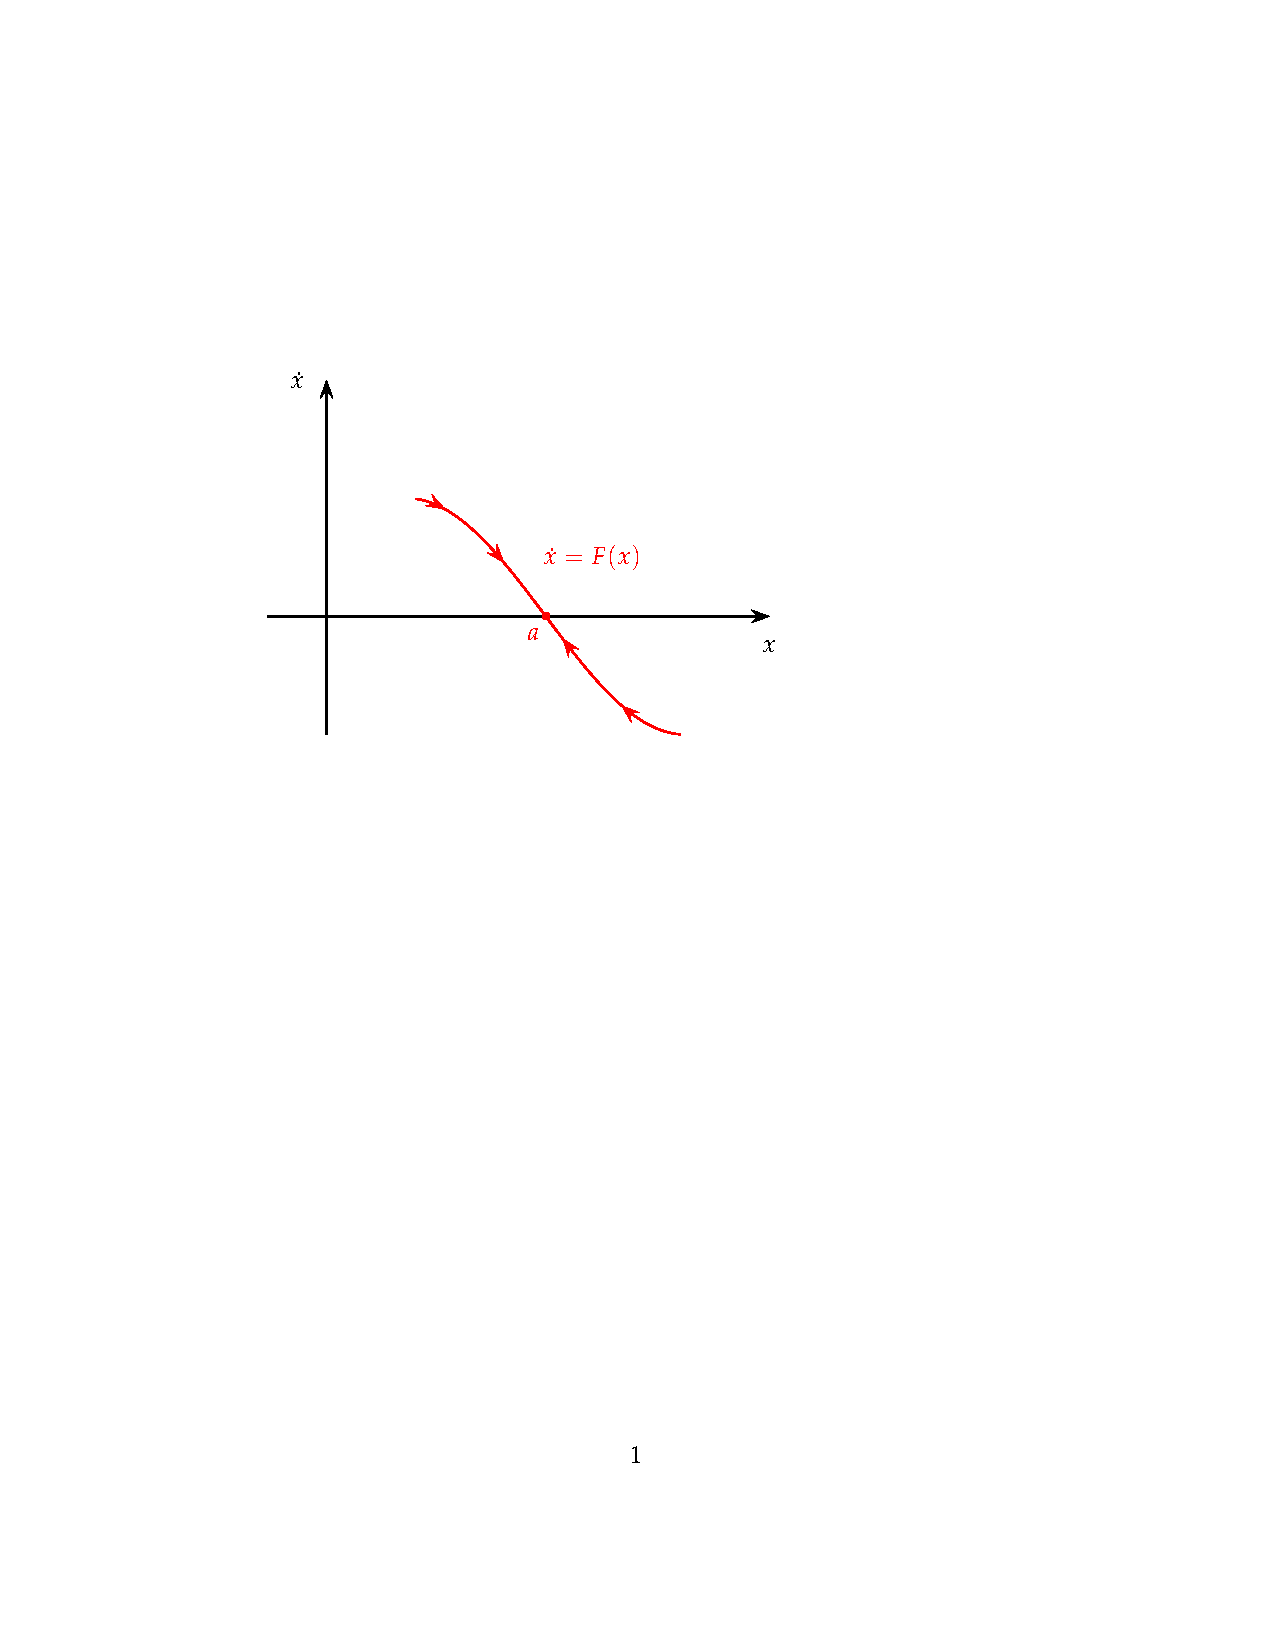
\includegraphics[scale=0.5]{graphs/phase1}
\end{center}
\begin{itemize}
	\item To the left of $a$, $\dot{x} > 0$, therefore $x$ is increasing; to the right of it, $\dot{x} < 0$, therefore $x$ is decreasing
\end{itemize}
\end{frame}

\begin{frame}[fragile]
\frametitle{Autonomous Equations and Stability (2)}
\begin{itemize}
	\item In the latter, the point $a$ is an equilibrium point as $F(a) = 0$
	\item In other words, $x$ is not changing at this point, it is stationary there
	\item The graph displays a case of \textit{globally asymptotically stable} equilibrium
	\item Explanation: $x$ will always return to equilibrium no matter where it starts from
	\item In the following graph, we have two different types of equilibria
\end{itemize}
\end{frame}

\begin{frame}[fragile]
\frametitle{Autonomous Equations and Stability (3)}
\begin{center}
	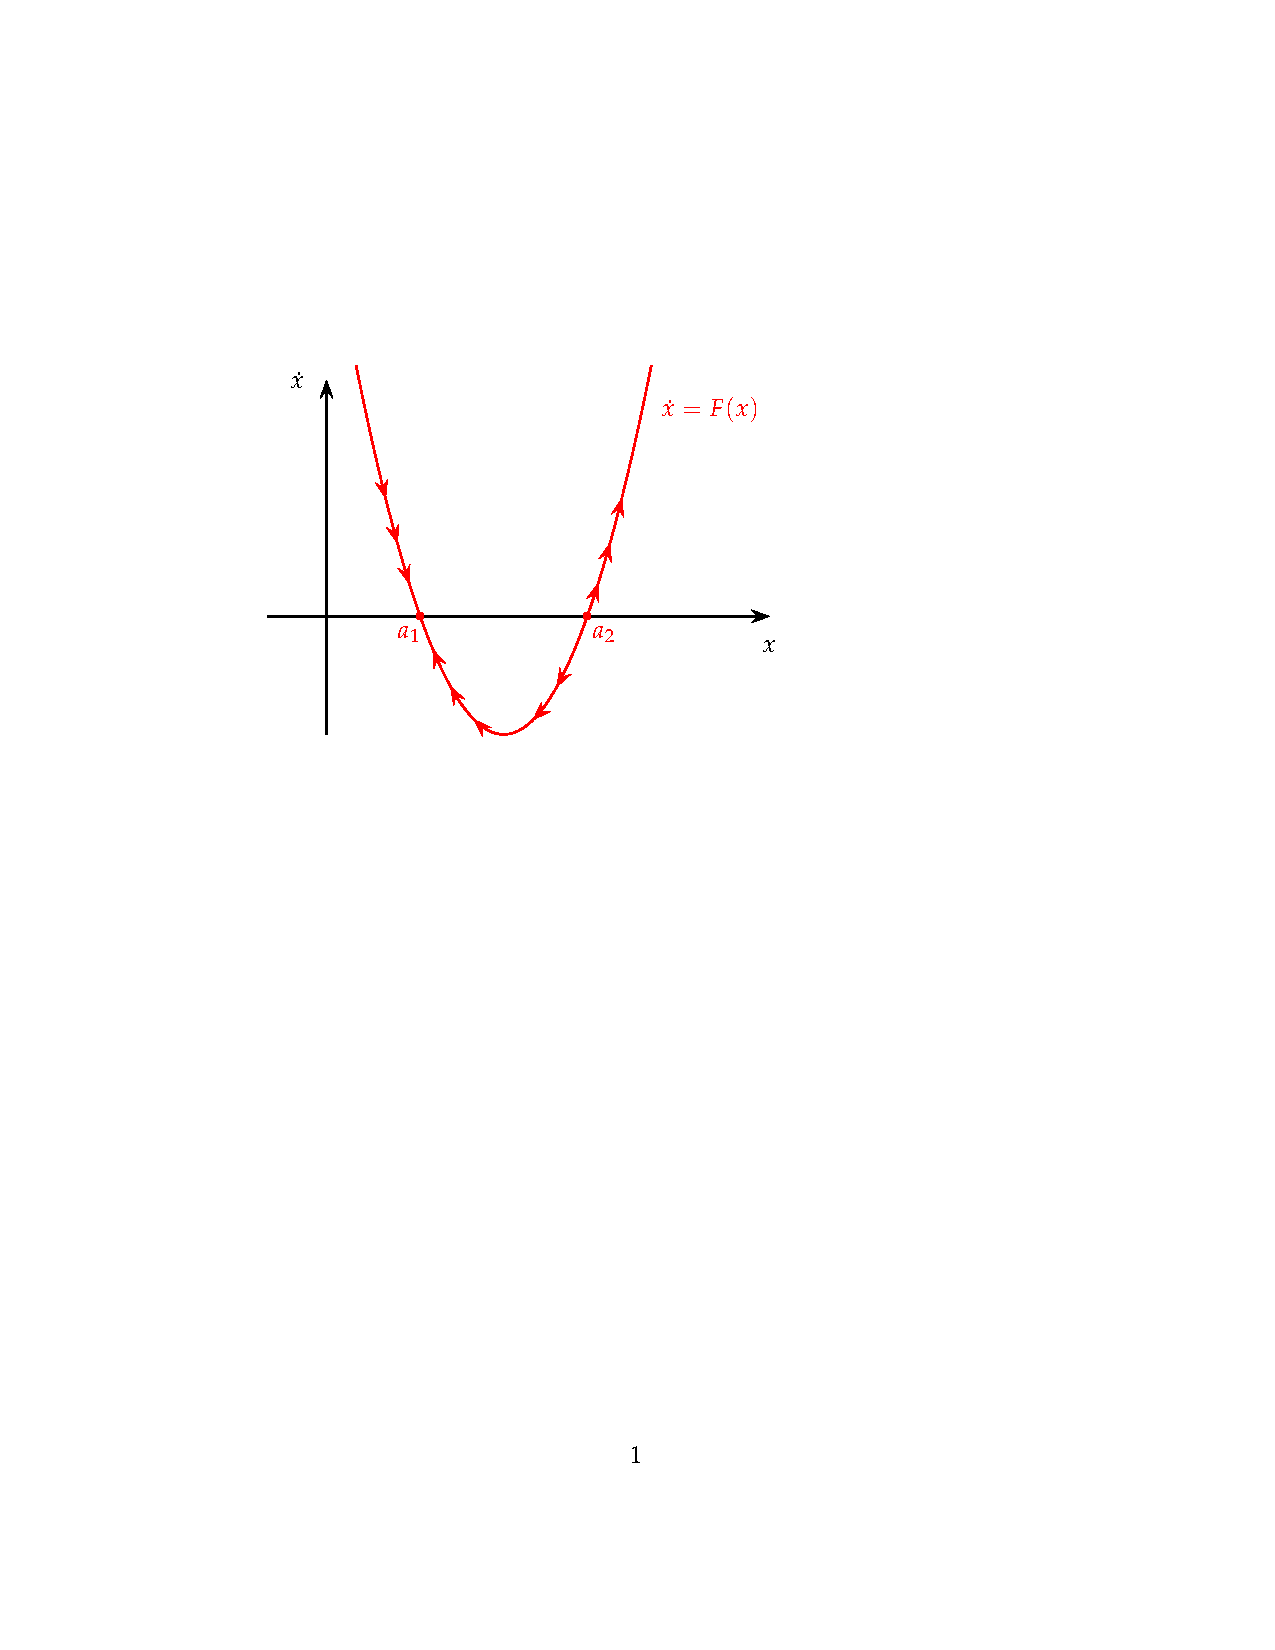
\includegraphics[scale=0.5]{graphs/phase2}
\end{center}
\begin{itemize}
	\item Here, $a_{1}$ is a \textit{locally stable equilibrium}, while $a_{2}$ is \textit{unstable}
\end{itemize}
\begin{block}{A summary of stability conditions}
\begin{itemize}
	\item $F(a)$ = 0 and $F'(a) < 0 \Rightarrow$ $a$ is locally stable
	\item $F(a)$ = 0 and $F'(a) > 0 \Rightarrow$ $a$ is unstable
	\item $F(a)$ = 0 and $F'(a) = 0 \Rightarrow$ inconclusive
\end{itemize}\end{block}
\end{frame}

\section{Existence and Uniqueness}
\begin{frame}[fragile]
\frametitle{Existence and Uniqueness}
\begin{theorem}
	Given the first-order ODE:
	\[
		\dot{x} = F(t,x),
	\]
	suppose that $F(t,x)$ and $F'_{x}(t,x)$ are continuous in an open set $A$ in the $tx$-plane. Take an arbitrary point $(t_{0},x_{0}) \in A$. Then there exists a unique ``local'' solution that passes through $(t_{0},x_{0})$.
\end{theorem}
\begin{itemize}
	\item ``local'' means that existence of solution is guaranteed for a small neighbourhood of $t_{0}$ only
\end{itemize}
\end{frame}

\begin{frame}[fragile]
\frametitle{Global Existence and Uniqueness}
\begin{theorem}
	Consider the initial-value problem:
	\[
		\dot{x} = F(t,x), \quad x(t_{0}) = x_{0}
	\]
	Suppose that $F(t,x)$ and $F'_{x}(t,x)$ are continuous $\forall (t,x)$. Suppose also there exist continuous functions $a(t)$ and $b(t)$ such that
	\[
		|F(t,x)| \leq a(t)|x| + b(t), \quad \forall (t,x)
	\]
	For an arbitrary point $(t_{0},x_{0})$ there exists a unique solution defined on $(-\infty,\infty)$. If the above condition is weakened to
	\[
		xF(t,x) \leq a(t)|x|^{2} + b(t), \quad \forall x \textrm{ and } \forall t \geq t_{0}
	\]
	then there is a unique solution of the problem on $[t_{0},+\infty)$.
\end{theorem}
\end{frame}

\section{Second-Order Equations}
\begin{frame}[fragile]
\frametitle{Second-Order Equations}
\begin{itemize}
	\item Typical second-order equations have the following form:
	\[
		\ddot{x} = F(t,x,\dot{x})
	\]
	\item A solution to that equation on an interval $I$ is a $C^{2}$ function that satisfies it
	\item A very simple example:
	\[
		\ddot{x}(t) = k,\quad k = const
	\]
	\item The solution with respect to the unknown function $x(t)$ is obtained after integrating the equation twice
\end{itemize}
\end{frame}

\begin{frame}[fragile]
\frametitle{Special Cases Where $x$ or $t$ is Missing}
\begin{itemize}
	\item \textcolor{darkred}{Case 1:} $x$ is missing in the RHS
	\[
		\ddot{x} = F(\dot{x},t)
	\]
	\item Solution: introduce a variable $u = \dot{x}$
	\item Then, the equation can be reduced to a first-order one, i.e.
	\[
		\dot{u} = F(u,t)
	\]
	\item After solving this for the unknown function $u(t)$, then we go to solve the first-order equation
	\[
		\dot{x} = u
	\]
	\color{orange}
	Example: $\ddot{x} = \dot{x} + t$
	\color{black}
\end{itemize}
\end{frame}

\begin{frame}[fragile]
\frametitle{Special Cases Where $x$ or $t$ is Missing (2)}
\begin{itemize}
	\item \textcolor{darkred}{Case 2:} $t$ is missing in the RHS
	\item In such a case, the equation is autonomous
	\item It can be transformed into an equation in terms of $t$ and then again reduced to a first-order equation
	\item Examples are left to your curiosity (see e.g. Problem 6 on p. 225)
\end{itemize}
\end{frame}

\begin{frame}[fragile]
\frametitle{Linear Second-Order ODE}
\begin{itemize}
	\item General form:
	\[
		\ddot{x} + a(t)\dot{x} + b(t)x = f(t)
	\]
	\item Unlike first-order equations, there is no explicit solution in the general case
	\item Nevertheless, the general structure of the solution can still be characterized
	\item Start with the homogeneous version of the above equation:
	\[
		\ddot{x} + a(t)\dot{x} + b(t)x = 0
	\]
	\item By the \textit{superposition principle}\footnote{\url{http://mathworld.wolfram.com/SuperpositionPrinciple.html}}, if $u_{1} = u_{1}(t)$ and $u_{2} = u_{2}(t)$ both satisfy the homogeneous equation, then $x = Au_{1} + Bu_{2}$ will also satisfy it, $\forall A,B$
\end{itemize}
\end{frame}

\begin{frame}[fragile]
\frametitle{Linear Second-Order ODE (2)}
\begin{itemize}
	\item Indeed, since $\dot{x} = A\dot{u}_{1} + B\dot{u}_{2}$ and $\ddot{x} = A\ddot{u}_{1} + B\ddot{u}_{2}$:
	\[
		\begin{array}{lcl}
			\ddot{x} + a(t)\dot{x} + b(t)x & = & A\ddot{u}_{1} + B\ddot{u}_{2} + a(t)(A\dot{u}_{1} + B\dot{u}_{2}) + b(t)(Au_{1} + Bu_{2}) = \\
			\quad\\
			& = & A[\ddot{u}_{1} + a(t)\dot{u}_{1} + b(t)u_{1}] + B[\ddot{u}_{2} + a(t)\dot{u}_{2} + b(t)u_{2}]
		\end{array}
	\]
	\item But since $u_{1}$ and $u_{2}$ satisfy the equation, then it is clear that the RHS of the latter equals 0
	\item This directly shows that $x = Au_{1} + Bu_{2}$ also satisfies it, $\forall A,B$
	\item However, $u_{1}$ and $u_{2}$ must not be proportional to each other
\end{itemize}
\end{frame}

\begin{frame}[fragile]
\frametitle{Linear Second-Order ODE (3)}
\begin{itemize}
	\item Suppose that a \textit{particular solution} $u^{*} = u^{*}(t)$ to the non-homogeneous equation can be found
	\item If $x(t)$ is an arbitrary solution of the non-homogeneous equation, then $x(t) - u^{*}(t)$ will be a solution to its homogeneous counterpart
	\item To see this, set $v = v(t) = x(t) - u^{*}(t)$
	\item Then, $\dot{v} = \dot{x} - \dot{u}^{*}$ and $\ddot{v} = \ddot{x} - \ddot{u}^{*}$, so that
	\[
		\begin{array}{lcl}
			\ddot{v} + a(t)\dot{v} + b(t)v & = & \ddot{x} - \ddot{u}^{*} + a(t)(\dot{x} - \dot{u}^{*}) + b(t)(x - u^{*}) = \\
			\quad\\
			& = & \ddot{x} + a(t)\dot{x} + b(t)x - [\ddot{u}^{*} + a(t)\dot{u}^{*} + b(t)u^{*}] = \\
			\quad\\
			& = & f(t) - f(t) = 0
		\end{array}
	\]
\end{itemize}
\end{frame}

\begin{frame}[fragile]
\frametitle{Linear Second-Order ODE (4)}
\begin{itemize}
	\item The latter showed that $x(t) - u(t)^{*}$ is a solution to the homogeneous equation
	\item But then we can write (using the above arguments) that:
	\[
		x(t) - u(t)^{*} = Au_{1}(t) + Bu_{2}(t)
	\]
	where $u_{1}(t)$ and $u_{2}(t)$ are two non-proportional solutions of the homogeneous equation, and $A$ and $B$ are two arbitrary constants
	\item The latter implies that if $x(t) - u(t)^{*}$ is a solution to the homogeneous equation, $x(t)$ is a solution to the non-homogeneous one
\end{itemize}
\end{frame}

\begin{frame}[fragile]
\frametitle{Linear Second-Order ODE (5)}
\begin{theorem}
	\begin{enumerate}
		\item[(a)] The \textbf{general solution} of the homogeneous equation is
		\[
			x(t) = Au_{1}(t) + Bu_{2}(t)
		\]
		where $u_{1}(t)$ and $u_{2}(t)$ are two non-proportional (linearly independent) solutions, and $A$ and $B$ are two arbitrary constants
		\item[(b)] The \textbf{general solution} of the non-homogeneous equation is
		\[
			x(t) = Au_{1}(t) + Bu_{2}(t) + u^{*}(t)
		\]
		where $Au_{1}(t) + Bu_{2}(t)$ is the general solution of the homogeneous equation, and $u^{*}(t)$ is any \textbf{particular solution} of the non-homogeneous equation
	\end{enumerate}
\end{theorem}
\end{frame}

\begin{frame}[fragile]
\frametitle{Constant Coefficients}
\begin{itemize}
	\item The homogeneous equation has the following form:
	\[
		\ddot{x} + a\dot{x} + bx = 0
	\]
	\item Using the theorem, we look for two non-proportional solutions $u_{1}(t)$ and $u_{2}(t)$
	\item Since the coefficients are constants, we try solutions such that $x$, $\dot{x}$, and $\ddot{x}$ are constant multiples of each other
	\item The function that has such a property is $x = e^{rt}$ (because $\dot{x} = re^{rt} = rx$ and $\ddot{x} = r^{2}e^{rt} = r^{2}x$)
\end{itemize}
\end{frame}

\begin{frame}[fragile]
\frametitle{Constant Coefficients (2)}
\begin{itemize}
	\item Substitute it in the equation:
	\[
		r^{2}e^{rt} + are^{rt} + be^{rt} = 0
	\]
	\item Divide both sides by $e^{rt} \neq 0$ to get
	\[
		r^{2} + ar + b = 0
	\]
	\item The latter is the \textit{characteristic equation} of the differential equation
	\item Finding the values of $r$ from it allows to find the solutions $x = e^{rt}$ that satisfy the homogeneous equation
\end{itemize}
\end{frame}

\begin{frame}[fragile]
\frametitle{Constant Coefficients (3)}
\begin{theorem}
	The \textbf{general solution} of the constant-coefficients homogeneous equation is determined by the roots of its characteristic equation as follows:
	\begin{enumerate}
		\item[(I)] If the discriminant $a^{2} - 4b > 0$, there are two distinct real roots, and:
		\[
			x = Ae^{r_{1}t} + Be^{r_{2}t}, \quad r_{1,2} = -\dfrac{a \pm \sqrt{a^{2} - 4b}}{2}  
		\]
		\item[(II)] If $a^{2} - 4b = 0$, then there is a double real root, and:
		\[
			x = (A + Bt)e^{rt}, \quad r = -\dfrac{a}{2}
		\]
		\item[(III)] If $a^{2} - 4b < 0$, then there are two complex conjugate roots $r_{1,2} = \alpha \pm \beta i$, and:
		\[
			x = e^{\alpha t}(A\cos \beta t + B\sin \beta t),\quad \alpha = -\dfrac{a}{2}, \, \beta = \dfrac{\sqrt{4b - a^{2}}}{2}
		\]
	\end{enumerate}
\end{theorem}
\end{frame}

\begin{frame}[fragile]
\frametitle{The Non-Homogeneous Equation}
\begin{itemize}
	\item Has the following form:
	\[
		\ddot{x} + a\dot{x} + bx = f(t)
	\]
	where $f(t)$ is an arbitrary continuous function 
	\item According to Theorem 3 (b), its general solution is:
	\[
		x(t) = Au_{1}(t) + Bu_{2}(t) + u^{*}(t)
	\]
	\item Finding two solutions $u_{1}(t)$ and $u_{2}(t)$ is clear from the homogeneous case
	\item What's needed is a method to find $u^{*}(t)$
\end{itemize}
\end{frame}

\begin{frame}[fragile]
\frametitle{The Non-Homogeneous Equation (2)}
\begin{itemize}
	\item One way is to use the \textit{method of undetermined coefficients}
	\item If $b = 0$, then the equation can be transformed into a first order one (after setting $u = \dot{x}$)
	\item Assuming $b \neq 0$, four special cases are discussed here
	\item \textbf{Case 1:} $f(t) = A = const$
	\item The first step is to check whether the particular solution is a constant, i.e. $u^{*} = c$
	\item If so, then $\dot{u}^{*} = \ddot{u}^{*} = 0$, and the equation reduces to $bc = A \Rightarrow c = A/b$
	\item Therefore, for $b \neq 0$ a particular solution of 
	\[
		\ddot{x} + a\dot{x} + bx = A
	\]
	is the constant function
	\[
		u^{*} = A/b
	\]
\end{itemize}
\end{frame}

\begin{frame}[fragile]
\frametitle{The Non-Homogeneous Equation (3)}
\begin{itemize}
	\item \textbf{Case 2:} $f(t)$ is a polynomial of degree $n$
	\item Then it is reasonable to assume that the solution is also a polynomial of degree $n$:
	\[
		u^{*} = A_{n}t^{n} + A_{n-1}t^{n-1} + \ldots + A_{1}t + A_{0}
	\]
	\item The coefficients $A_{n}, A_{n-1},\ldots,A_{0}$ are determined so that $u^{*}$ is required to satisfy the non-homogeneous equation and the coefficients of like powers of $t$ are equated
	\item \textcolor{red}{Example: solve $\ddot{x} - 4\dot{x} + 4x = t^{2} + 2$}
\end{itemize}
\end{frame}

\begin{frame}[fragile]
\frametitle{The Non-Homogeneous Equation (4)}
\begin{itemize}
	\item \textbf{Case 3:} $f(t) = pe^{qt}$
	\item A solution of the form $u^{*} = Ae^{qt}$ is tried
	\item With this, $\dot{u}^{*} = Aqe^{qt}$ and $\ddot{u}^{*} = Aq^{2}e^{qt}$
	\item Substituting the latter two into the equation leads to:
	\[
		Ae^{qt}(q^{2} + aq + b) = pe^{qt}
	\]
	\item Three possibilities exist:
	\begin{enumerate}
		\item $q^{2} + aq + b \neq 0$, i.e. $q$ is not a solution of the characteristic equation (in other words, $e^{qt}$ is not a solution of the homogeneous equation)
		\item $q$ is a simple root of $q^{2} + aq + b = 0$
		\item $q$ is a double root of $q^{2} + aq + b = 0$
	\end{enumerate}
\end{itemize}
\end{frame}

\begin{frame}[fragile]
\frametitle{The Non-Homogeneous Equation (5)}
\begin{itemize}
	\item In case 3.1, the particular solution of the equation $\ddot{x} + a\dot{x} + bx = pe^{qt}$ is
	\[
		u^{*} = \dfrac{p}{q^{2} + aq + b}e^{qt}
	\]
	\item In case 3.2, a constant $B$ is sought such that $Bte^{qt}$ is a solution
	\item In case 3.3, a constant $C$ is sought such that $Ct^{2}e^{qt}$ is a solution
\end{itemize}
\end{frame}

\begin{frame}[fragile]
\frametitle{The Non-Homogeneous Equation (6)}
\begin{itemize}
	\item \textbf{Case 4:} $f(t) = p\sin (rt) + q\cos (rt)$
	\item The method of undetermined coefficients is used again
	\item Let $u^{*} = A\sin (rt) + B\cos (rt) $
	\item The constants $A$ and $B$ are adjusted so that the coefficients of $\sin rt$ and $\cos rt$ match
	\item If $f(t)$ is itself a solution of the homogeneous equation, then for suitable choices of $A$ and $B$, the particular solution equals:
	\[
		u^{*} = At\sin (rt) + Bt\cos (rt)
	\]
\end{itemize}
\end{frame}

\begin{frame}[fragile]
\frametitle{Stability}
\begin{block}{Stability}
	The equation
	\[
		\ddot{x} + a\dot{x} + bx = f(t)
	\]
	is \textit{globally asymptotically stable} iff both roots of its characteristic equation have negative real parts.
\end{block}
\begin{itemize}
	\item Note that this result extends to equations of higher order
	\item That an equation is globally asymptotically stable means that every solution $Au_{1}(t) + Bu_{2}(t)$ of the associated homogeneous equation tends to 0 as $t\to\infty$, $\forall A,B$
\end{itemize}
\end{frame}

\section{Systems of Differential Equations}
\begin{frame}[fragile]
	\frametitle{Systems of Differential Equations}
	\begin{itemize}
		\item \textit{Normal form} for systems of differential equations:
		\[
			\left|
			\begin{array}{lcl}
				\dot{x}_{1} & = & f_{1}(t, x_{1}, x_{2},\ldots,x_{n})\\
				\dot{x}_{2} & = & f_{2}(t, x_{1}, x_{2},\ldots,x_{n})\\
				\hdotsfor{3}\\
				\dot{x}_{n} & = & f_{n}(x_{1}, x_{2},\ldots,x_{n})\\
			\end{array}\right. \quad (\spadesuit)
		\]
		
		\item In other words, derivatives should be located only in the LHSs of equations
		
		\item Also, there is one derivative per equation
		
		\item Finally, all derivatives are first-order only
	\end{itemize}
\end{frame}

\begin{frame}[fragile]
	\frametitle{Systems of Differential Equations (2)}
	\begin{itemize}
		\color{blue}
		\item Example of a system of differential equations:
		\[
			\left|
			\begin{array}{lcl}
				\ddot{x}_{1} & = & F_{1}(t, x_{1}, x_{2},\dot{x}_{1}, \dot{x}_{2})\\
				\ddot{x}_{2} & = & F_{2}(t, x_{1}, x_{2},\dot{x}_{1}, \dot{x}_{2})\\
			\end{array}\right.
		\]
		
		\color{black}
		\item This system is \textit{not} in normal form!
		
		\item To transform it to a normal form, introduce new variables:
		\[
			u_{1} = x_{1}, \quad u_{2} = x_{2}, \quad u_{3} = \dot{x}_{1}, \quad u_{4} = \dot{x}_{2}
		\]
		
		\item The system becomes
		\[
		\left|
		\begin{array}{lcl}
			\dot{u}_{1} & = & u_{3}\\
			\dot{u}_{3} & = & f_{1}(t, u_{1}, u_{2}, u_{3}, u_{4})\\
			\dot{u}_{2} & = & u_{4}\\
			\dot{u}_{4} & = & f_{2}(t, u_{1}, u_{2}, u_{3}, u_{4})\\	
		\end{array}\right.
		\]
	\end{itemize}
\end{frame}

\begin{frame}[fragile]
	\frametitle{Systems of Differential Equations (3)}
	\begin{itemize}
		\item A set of functions $ x_{1} = x_{1}(t), x_{2} = x_{2}(t), \ldots, x_{n} = x_{n}(t) $ that satisfies the system $ (\spadesuit) $ is called a \textit{solution}
		
		\item In $ \mathbb{R}^{n} $ the graph of the solution is a surface
		
		\item The vector $ \dot{\mathbf{x}}(t) = (\dot{x}_{1}(t), \dot{x}_{2}(t), \ldots, \dot{x}_{n}(t))$ is called the \textit{velocity vector}
		
		\item The space spanned by all vectors $ (x_{1}(t), x_{2}(t), \ldots, x_{n}(t)) $ is called the \textit{phase space}
		
		\item If all functions $ f_{i}(t, x_{1}(t), x_{2}(t),\ldots, x_{n}(t)) $ are collected in a vector $ \mathbf{F}(t, \mathbf{x}(t)) $, then the system of differential equations can be written as
		\[
			\dot{\mathbf{x}}(t) = \mathbf{F}(t, \mathbf{x}(t))
		\]
	\end{itemize}
\end{frame}

\begin{frame}[fragile]
	\frametitle{Systems of Differential Equations (4)}
	\begin{itemize}
		\item In economics the functions $ x_{1}(t), x_{2}(t), \ldots, x_{n}(t) $ are called \textit{state variables} as they describe the state of the economy at each time
		
		\item If the state of the economy at some time $ t_{0} $ is given, i.e. 
		\[
			\mathbf{x}(t_{0}) = (x_{1}(t_{0}), x_{2}(t_{0}), \ldots, x_{n}(t_{0}))
		\]
		
		is known, the specific solution of the system passing through this point could be found
		
		\item Existence and uniqueness of the solution is guaranteed by the condition that $ f_{i} $ and $ \dfrac{\partial f_{i}}{\partial x_{j}} $ are all continuous for $ i,j = 1,2,\ldots,n $
	\end{itemize}
\end{frame}

\begin{frame}[fragile]
	\frametitle{Linear Systems}
	\begin{itemize}
		\item General form:
		\[
			\left|
			\begin{array}{lcl}
				\dot{x}_{1}(t) & = & a_{11}(t)x_{1}(t) + a_{12}(t)x_{2}(t) + \ldots + a_{1n}(t)x_{n}(t) + b_{1}(t)\\
				\dot{x}_{2}(t) & = & a_{21}(t)x_{1}(t) + a_{22}(t)x_{2}(t) + \ldots + a_{2n}(t)x_{n}(t)+ b_{2}(t)\\
				\hdotsfor{3}\\
				\dot{x}_{n}(t) & = & a_{n1}(t)x_{1}(t) + a_{n2}(t)x_{2}(t) + \ldots + a_{nn}(t)x_{n}(t) + b_{n}(t)
			\end{array}\right.
		\]
		
		\item Using matrix notation, the latter can also be written as
		\[
			\dot{\mathbf{x}}(t) = \mathbf{A}(t)\mathbf{x}(t) + \mathbf{b}(t)
		\]
		
		\item If the coefficients $ a_{ij}, \ i,j = 1,2,\ldots,n $ are all constants, then the equation becomes
		\[
			\dot{\mathbf{x}}(t) = \mathbf{A}\mathbf{x}(t) + \mathbf{b}(t) \quad (\diamondsuit)
		\]
		
		\item Equations of this type can always be solved explicitly
	\end{itemize}
\end{frame}

\begin{frame}[fragile]
	\frametitle{Linear Systems (2)}
	\begin{itemize}
		\item The system defined by $ (\diamondsuit) $ is globally asymptotically stable if and only if all the eigenvalues of $ \mathbf{A} $ have negative real parts
		
		\item Assume that the system is autonomous, i.e.
		\[
			\dot{\mathbf{x}}(t) = \mathbf{A}\mathbf{x}(t) + \mathbf{b}
		\]
		
		\item To solve it based on eigenvalues, first consider its homogeneous counterpart:
		\[
			\dot{\mathbf{x}}(t) = \mathbf{A}\mathbf{x}(t)
		\]
		
		\item The goal is to find numbers $ \lambda $ and $ v_{1}, v_{2},\ldots,v_{n} $ such that the vector function $ \mathbf{x} = \mathbf{v}e^{\lambda t} $ satisfies the homogeneous system
	\end{itemize}
\end{frame}

\begin{frame}[fragile]
	\frametitle{Linear Systems (3)}
	\begin{itemize}
		\item Differentiate $ \mathbf{x} = \mathbf{v}e^{\lambda t} $ with respect to $ t $:
		\[
			\dot{\mathbf{x}}(t) = \lambda\mathbf{v}e^{\lambda t}
		\]
		
		\item Then the homogeneous system becomes
		\[
			\lambda\mathbf{v}e^{\lambda t} = \mathbf{A} \mathbf{v}e^{\lambda t}  \Rightarrow \mathbf{A} \mathbf{v} = \lambda\mathbf{v} 
		\]
		
		\item The latter implies that any non-zero solution is an eigenvector of $ \mathbf{A} $ with a corresponding eigenvalue $ \lambda $
		
		\item If $ \mathbf{A} $ has $ n $ different eigenvalues then the general solution of the homogeneous system is
		\[
			\mathbf{x}(t) = C_{1}e^{\lambda_{1}t}\mathbf{v}_{1} + C_{2}e^{\lambda_{2}t}\mathbf{v}_{2} + \ldots +  C_{n}e^{\lambda_{n}t}\mathbf{v}_{n}
		\]
	\end{itemize}
\end{frame}

\begin{frame}[fragile]
	\frametitle{Linear Systems (4)}
	\begin{itemize}
		\item Concerning the solution of the non-homogeneous system, if $ \mathbf{x}^{0} $ is an equilibrium point, then 
		\[
			\mathbf{Ax}^{0} + \mathbf{b} = \mathbf{0}
		\]
		
		\item Define the deviation of $ \mathbf{x}(t) $ from this equilibrium point as
		\[
			\mathbf{w}(t) = \mathbf{x}(t) - \mathbf{x}^{0}
		\]
		
		\item Clearly, $ \dot{\mathbf{w}} = \dot{\mathbf{x}} $, and therefore
		\[
			\dot{\mathbf{w}}(t) = \mathbf{A}\mathbf{x}(t) + \mathbf{b} \Leftrightarrow \dot{\mathbf{w}}(t) = \mathbf{A}(\mathbf{w}(t) + \mathbf{x}^{0}) + \mathbf{b}
		\]
		
		\item Uncover the parentheses in the far RHS:
		\[
			\dot{\mathbf{w}}(t) = \mathbf{A} \mathbf{w}(t) + \textcolor{red}{\underbrace{\mathbf{A}\mathbf{x}^{0} + \mathbf{b}}_{=\mathbf{0}}} =  \mathbf{A} \mathbf{w}(t)
		\]
		i.e. the non-homogeneous system can be transformed into a homogeneous one
	\end{itemize}
\end{frame}

\begin{frame}[fragile]
\frametitle{References}
\begin{itemize}
	\item Chiang, A., and K. Wainright (2004): \textit{Fundamental Methods of Mathematical Economics}, McGraw-Hill, 4th ed., ch. 15, 16, 19
	\item Shone, R. (2002): \textit{Economic Dynamics: Phase Diagrams and Their Economic Application}, Cambridge University Press, 2nd ed., ch. 2, 4
	\item Syds{\ae}ter, K., P. Hammond, A. Seierstad, and A. Str{\o}m (2008): \textit{Further Mathematics for Economic Analysis}, Prentice Hall, 2nd ed., ch. 5, 6, 7 
\end{itemize}
\end{frame}

\end{document}
	


